 \documentclass{common/nak}

%Deckblattkonfiguration
%Die Werte in den Klammern können entsprechend angepasst werden
\def\transferLeistungnnummer{69}
\def\matrikelNummer{42069}
\def\themenBeschreibung{Irgendein langweiliger shit der nichts mit Informatik zutun hat}
\def\studienGang{Angewandte Informatik}
\def\zenturie{A18a}

%General stuff
\usepackage{acronym}
\graphicspath{{images/}}
\usepackage{url}
\usepackage{outlines}
\usepackage{todonotes}
\usepackage{amsmath}
\numberwithin{equation}{subsection}

%%% --- The following two lines are what needs to be added --- %%%
\setcounter{biburllcpenalty}{7000}
\setcounter{biburlucpenalty}{8000}
\addbibresource{quellen.bib}

\begin{document}
\hspace{3cm}
%eigenes deckblatt
\begin{center}
    
\includegraphics[width=0.7\textwidth]{images/nak_logo2.png}\\
     \huge { Bachelorarbeit \\[1em]
     \large{Analyse der Effektivität von Media-Kanälen zur Steigerung der Nachfrage:
     \\ Eine Untersuchung mit Marketing-Mix-Modell bei bonprix Handelsgesellschaft mbH
}}
\end{center}

\vspace*{\fill}


\noindent Vorgelegt von:\\
Enxi Hong \\
Zeisigring \\
24568 Kaltenkirchen\\
E-Mail: enxi.hong@nordakademie.de\\
\\
Matrikelnummer: 11952\\
Jahrgang: 2021\\
Studiengang: Angewandte Informatik\\
Datum: \today\\
Betreuender Dozent: Michael Fretschner\\

\newpage

%Seitenzahlen auf Römisch
\pagenumbering{Roman}

%Auskommentiert, weil expose
\iffalse
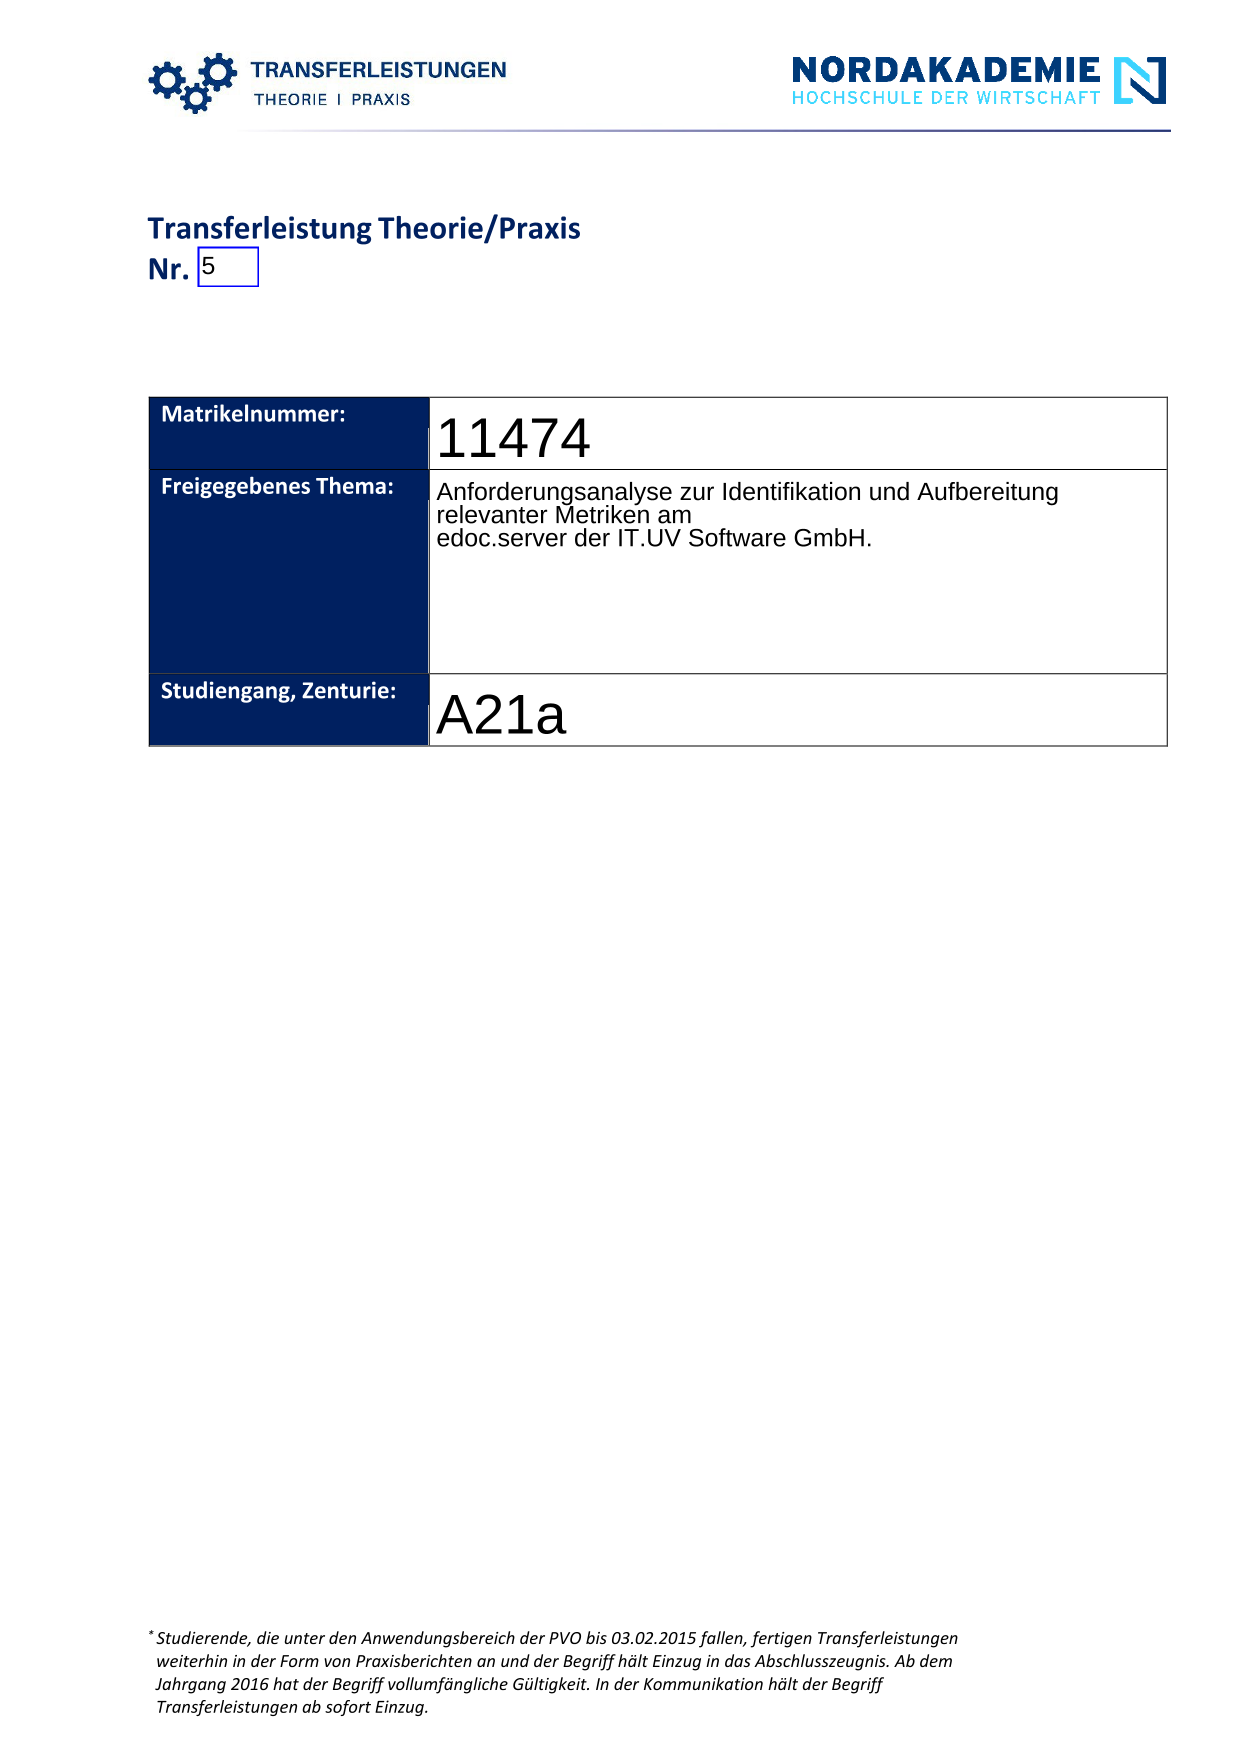
\includepdf{common/Transferleistung_Deckblatt_05_flattend}
\fi


\newpage
\section*{Sperrvermerk}

Die vorliegende Transferleistung beinhaltet interne vertrauliche Informationen der IT.UV Software GmbH. Die Weitergabe des Inhaltes der Arbeit und eventuell beiliegender Zeichnungen und Daten im Gesamten oder in Teilen ist grundsätzlich untersagt. Es dürfen keinerlei Kopien oder Abschriften - auch in digitaler Form - gefertigt werden. Ausnahmen bedürfen der schriftlichen Genehmigung der IT.UV Software GmbH.

\newpage

%Inhaltsverzeichnis
\tableofcontents
\newpage


\listoffigures
\addcontentsline{toc}{section}{Abbildungsverzeichnis}
%auskommentiert, wenn leer:

\newpage
\listoftables
\addcontentsline{toc}{section}{Tabellenverzeichnis}

\newpage
\addcontentsline{toc}{section}{Abkürzungsverzeichnis}
\addtocontents{toc}

\section*{Abkürzungsverzeichnis}
\begin{acronym}[Abkürzung] % Für Formatierung längste Abkürzung eintragen
\acro{ac:Label}[Abkürzung]{Langform}
\acro{MMM}{Marketing-Mix-Modell}
\acro{ROAS}{Return on Advertising Spend}
\acro{ROI}{Return on Investment}
\acro{olv}{Online Video}
\acro{dooh}{Digital Out of Home}
\acro{ooh}{Out of Home}
\acro{MLR}{Multiple linear Regression}
\acro{LAD}{Least Absolute Deviations}
\acro{OLS}{Ordinary Least Squares}
\acro{MLE}{Maximum Likelihood Estimation}
\acro{RSS}{Residual Sum of Squares}
\acro{PR}{Public Relations}
\acro{KPI}{Key Performance Indicators}
\acro{VIF}{Variance Inflation Factor}
\acro{SST}{Total Sum of Squares}
\acro{SSM}{Model Sum of Squares}
\acro{ToFu}{Top of the Funnel}
\acro{MoFu}{Middle of the Funnel}
\acro{BoFu}{Bottom of the Funnel}
\acro{SEA}{Search Engine Advertising}
\acro{OMA}{Online-Marketing}



%.u..
\end{acronym}
 

\newpage

\setcounter{page}{1}
%Seitenzahlen
\pagenumbering{arabic}
%Abbildungscounter sonst bei 2
\setcounter{figure}{0}

%Sectionen hinzufügen
\foreach \i in { 01, 02, 03, 04, 05, 06, 07, 08, 99 } {%
    \edef\FileName{sections/file\i}%
    \IfFileExists{\FileName}{%
       \input{\FileName}%
    }
}


%Quellen
\newpage
\clearpage
\printbibliography

\newpage
%Anhang
\appendix
\section*{Anhang}
\addcontentsline{toc}{section}{Anhang}



\iffalse
\subsection*{Anhang 1}
\label{anhang:Ersterhebung}
\addcontentsline{toc}{subsection}{Anhang 1}
Anforderungen aus der Ersterhebung:
\begin{center}
    \includegraphics[height=0.88\textheight]{images/Metriken_ersterhebung_manuell.png}
\end{center}

\newpage
\subsection*{Anhang 2}
\label{anhang:gruppiert}
\addcontentsline{toc}{subsection}{Anhang 2}
Metriken nach Gruppierung und Konfliktlösung:
\begin{center}
    \includegraphics[width=1\textwidth]{images/Metriken_Gruppiert_manuell.png}
\end{center}
\fi

\newpage
\end{document}
